This section describes a messaging architecture enabling the integration of the IMP solution described in the previous section into the existing OZG system architecture.

\subsection{Integration Overview}

\begin{center}
    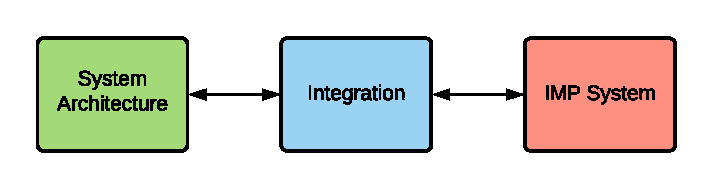
\includegraphics[scale=0.6]{Diagrams/Integration Architecture 1/Technological Integration/1. Integration Overview.pdf}
\end{center}

The IMP solution described in the previous section requires the administration portal to access IMP services. For integration, an IMP connector and a messaging system are added to the portal domain. Using the messaging system, existing systems of the administration portal can access IMP services trough the IMP connector.

\begin{center}
    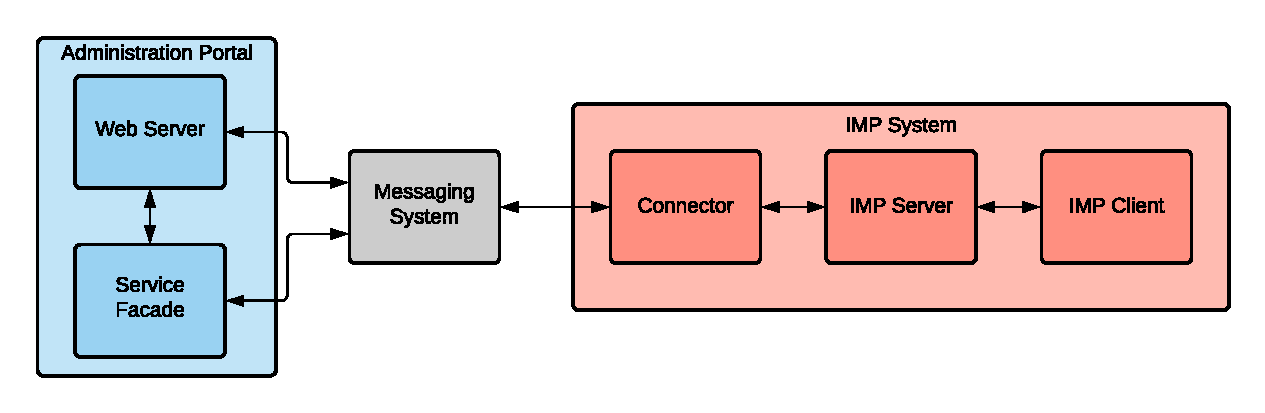
\includegraphics[scale=0.6]{Diagrams/Integration Architecture 1/Technological Integration/2. System Integration Overview.pdf}
\end{center}

In order for the integration not to be invasive, only the web server and the service facade of the administration portal are connected to the messaging system. All other existing system components remain untouched.

\subsection{Onboarding Sequence}

\begin{center}
    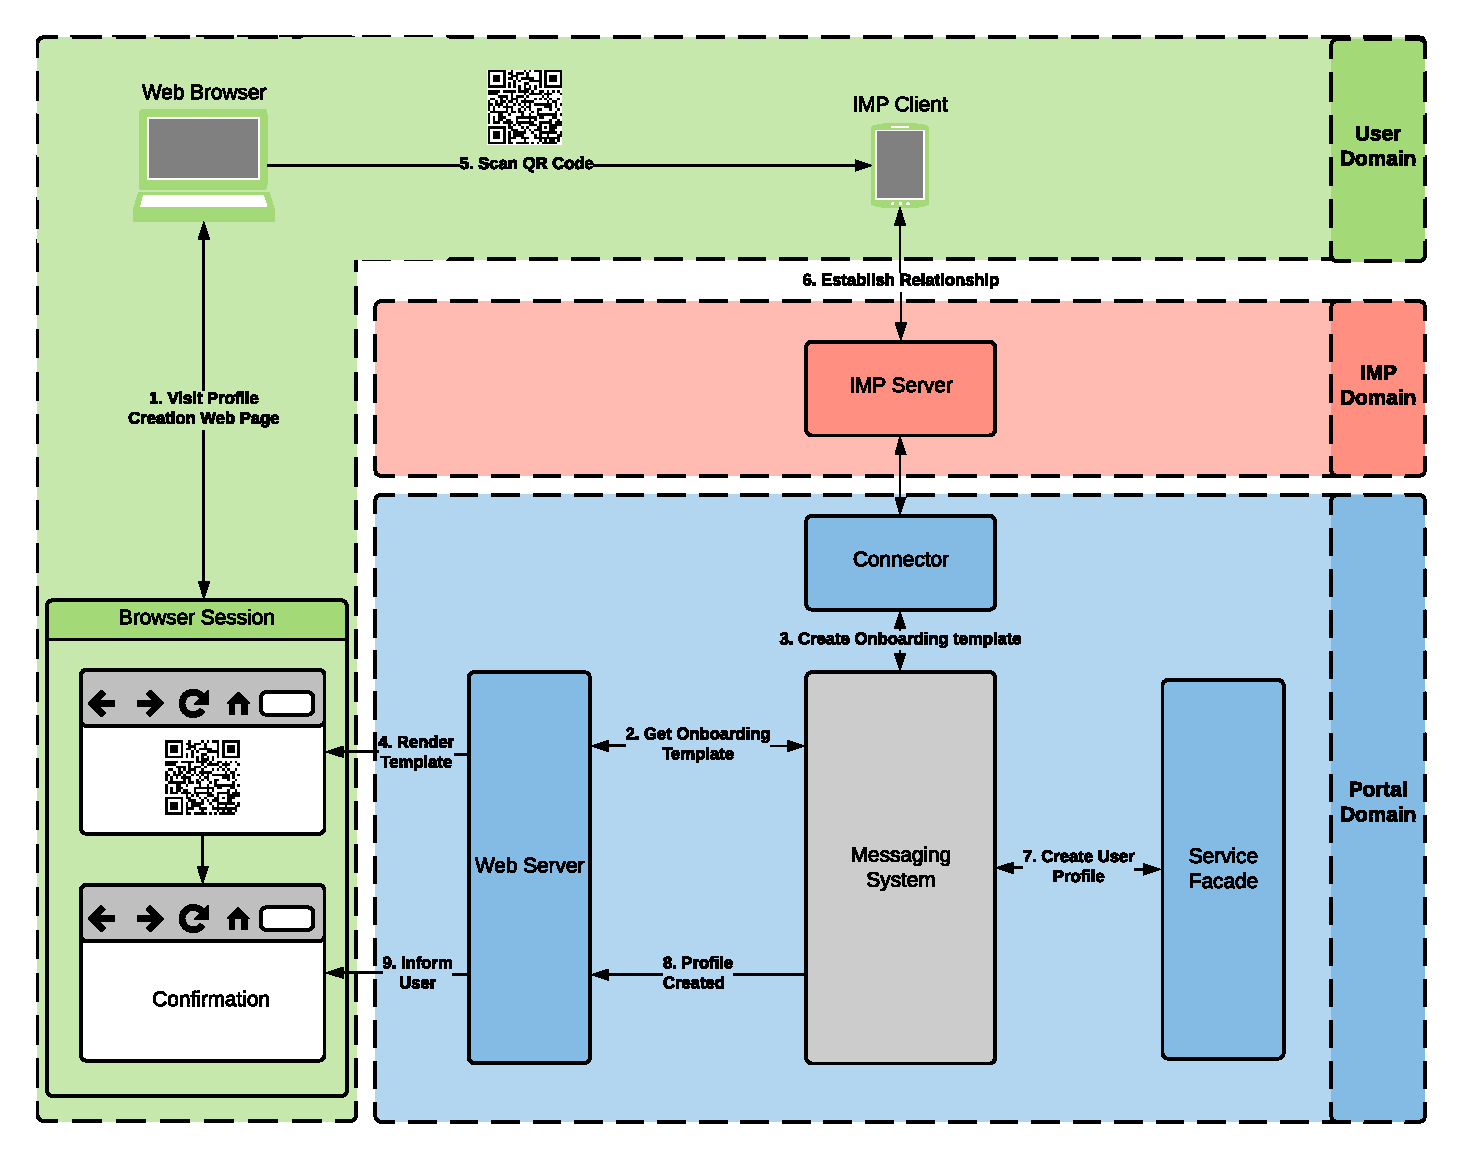
\includegraphics[scale=0.6]{Diagrams/Integration Architecture 1/Technological Integration/5. Onboarding Overview.pdf}
\end{center}

As described in section 5.1, the user should be able to create a new user profile for the OZG system through an existing IMP identity.

On the existing website of the administration portal, where users can create a user profile, the relationship template for onboarding should be displayed. When the web server receives a GET request for the profile creation website, it issues a request to the messaging system for a new onboarding template. The messaging system interacts with the IMP connector to construct the template and send it back to the web server. The web server renders the template as a QR code. The QR code is displayed on the device of the user who can use the IMP client to scan it and initiate a relationship request. The messaging system interacts with the connector to establish the relationship and eventually issues the service facade to create a new user profile based on the attributes shared as part of the IMP relationship. After successful creation of the user profile, the messaging system stores the relationship ID and the user profile ID in a database. In the future, each request containing either a user profile ID or relationship ID can be mapped to the correct OZG and IMP identities. The messaging system notifies the web server of the successful creation of the user profile and the web server displays a corresponding notification to the user.

\subsection{Messaging Overview}

\begin{center}
    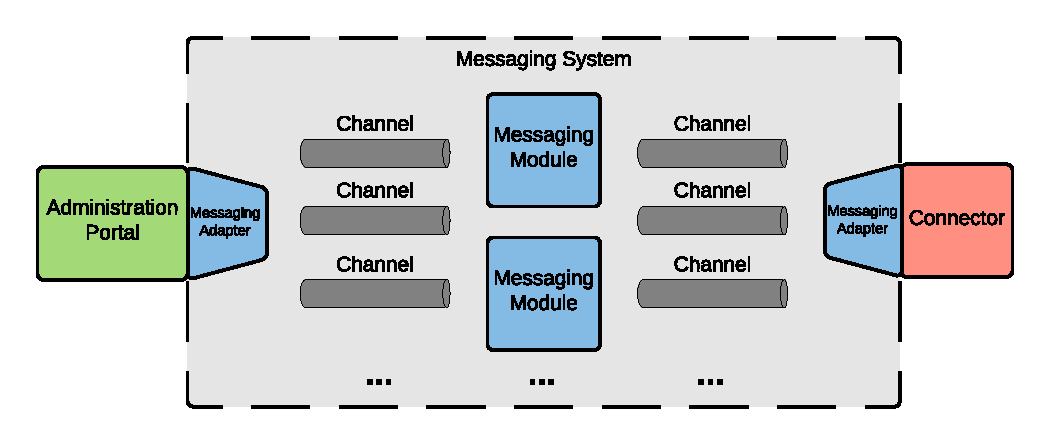
\includegraphics[scale=0.6]{Diagrams/Integration Architecture 1/Technological Integration/3. Messaging Integration.pdf}
\end{center}

The main task of the integration system is to translate between the domain of the existing system architecture and the domain of the IMP system. None of the existing systems can process IMP relationships but they can process user profiles and vice versa. 

On the side of the administration portal, messaging adapters provide an API to the existing systems providing access to IMP services while hiding the technological details of the operation of the IMP system and the underlying messaging system. The adapters communicate with the messaging system trough publish-subscribe datatype channels. Each datatype channel contains messages with the same datatype and has a defined purpose. All systems, consuming messages from the channel are aware of this purpose and process consumed messages accordingly. Messages placed on a publish-subscribe channel can be simultaneously accessed by multiple systems which subscribed to the channel. Using these channels, message adapters can send requests, receive replies, receive notifications, receive requests and send replies. 

On the side of the connector, messaging adapters translate the REST API of the connector to a set of publish-subscribe datatype channels. Using these channels, the messaging system can send REST requests by placing messages on channels corresponding to a certain interface. This also enables the messaging system to receive events from by the connector by the messaging adapter placing messages on a notification channels.

Messaging adapters do not communicate directly trough channels, but with messaging modules. Messaging modules consist of messaging patterns which are able to modify, delete and route messages. Purpose of the modules is to translate messages sent by messaging adapters of either service provider or connector to be understood by the respective recipient. Each module is assigned to an individual integration task. By adding or removing modules, integration capabilities of the messaging system can be suited to the system architecture of the service provider. Modules can be designed to provide services to messaging adapters or other modules. Designing modules specifically for the usage by other modules helps in distributing integration responsibilities and avoiding a single monolithic integration component.

\begin{center}
    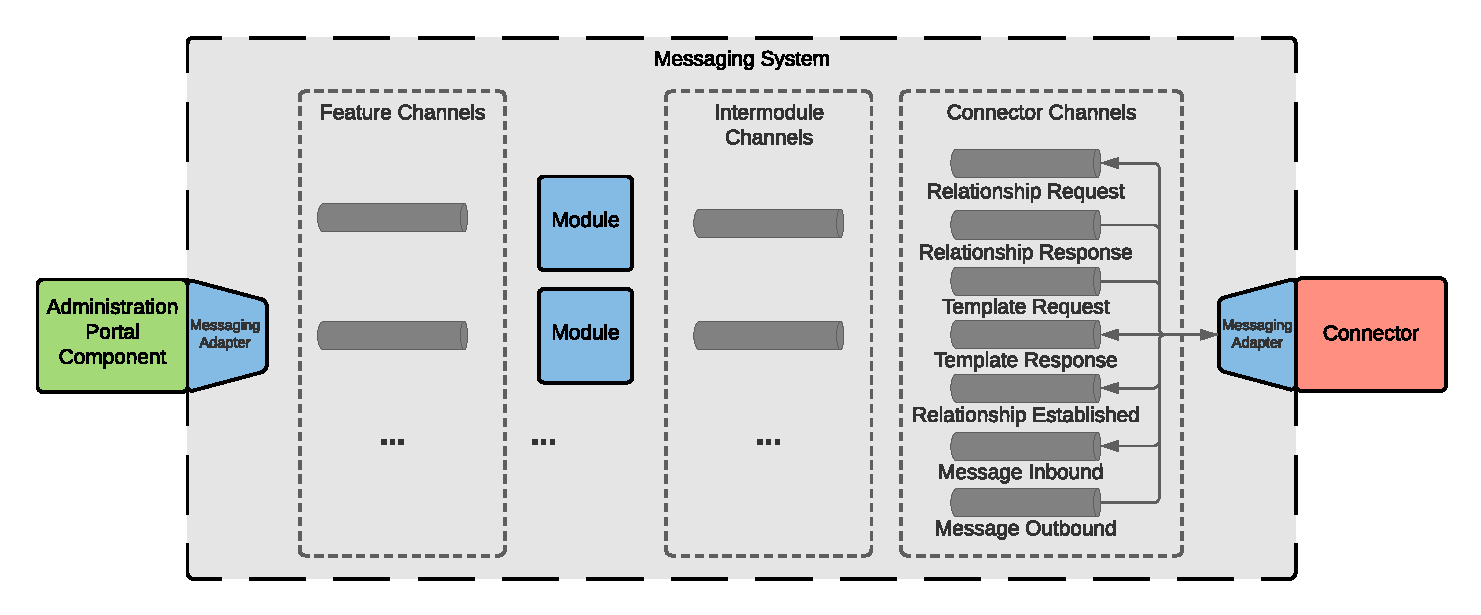
\includegraphics[scale=0.5]{Diagrams/Integration Architecture 1/Technological Integration/4. Messaging Overview.pdf}
\end{center}

The figure gives an overview of the messaging system which will be discussed in detail in the following sections. The figure contains all channels and messaging modules along with their connectivity.

As introduced in the beginning of this chapter, the technological integration can be separated into two layers: The "Relationship to Identity Integration Layer" and the "Communication Integration Layer" which is built upon it. As described in section 2.2, communication between IMP identity and service provider is only possible trough an established relationship.

Three messaging modules on the "Relationship to Identity Integration Layer" exist, which directly access services of the connector. The onboarding template module provides the feature of creating relationship templates for onboarding. The Onboarding request module, provides the feature of processing and responding to relationship requests. And the Onboarding relationship module provides the feature of processing established relationships by creating a new user profile. The relationship mapping module has the purpose of combining "Relationship to Identity Integration Layer" and "Communication Integration Layer" by enabling the messaging system to map relationships to the corresponding entity of the service provider. In this case, the module maps IDs of relationships to IDs of user profiles. Each relationship has a one-to-one relationship to a user profile.

The "Communication Integration Layer" consists of modules, which enable the existing systems to exchange structured data with the IMP client. Purpose of the modules is to translate between the data models of the service provider and the IMP system. Most importantly in this case, none of the existing systems is able to understand relationships or relationship IDs. Therefore, the message mapping module has the purpose of translating all incoming relationship IDs to user profile IDs with the help of the previously mentioned relationship mapping module on the underlying layer. Three message modules are included. Each of them has the purpose of identifying messages of a certain type and separate them on individual channels. This enables the construction of various modules processing the same message types in different ways. However, in this case, each message type has only a single module processing it. Modules which eventually process the messages, have the purpose of translating the message content between the data models of service provider and IMP system. For example the mail module consumes messages which contain a mail received by a user profile. It is very likely, that the inbox of the user profile and the inbox of the IMP system process mails with different data representation and data types. The mail module therefore has to convert the format of the mail content.

\subsection{Onboarding Template Module}

\begin{center}
    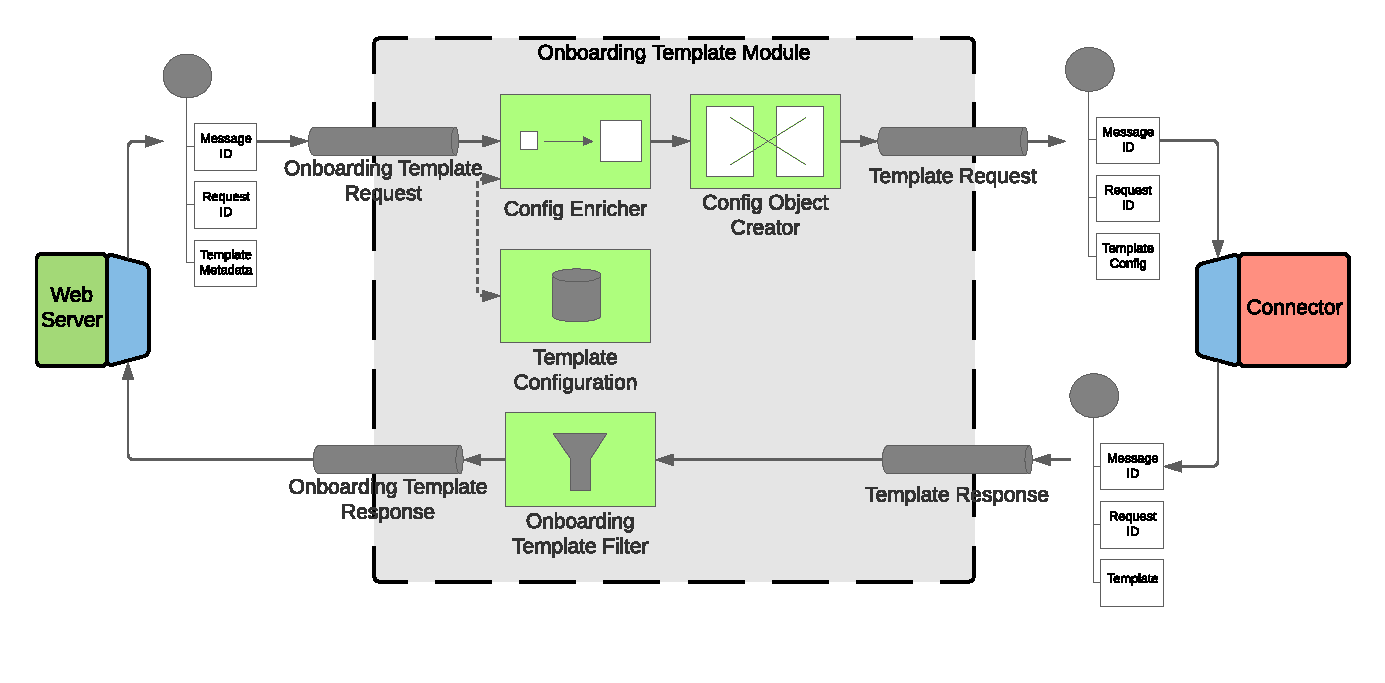
\includegraphics[scale=0.6]{Diagrams/Integration Architecture 1/Technological Integration/6. Onboarding Template Module.pdf}
\end{center}

To present an onboarding relationship template to the user, the web server first has to retrieve it from the messaging system. For this purpose, an "Onboarding Template Module" is added to the messaging system. Using the API of a messaging adapter provided in addition to the module, the web server can request the creation of new onboarding templates. Optionally, the web server can pass additional attributes which should be stored in the metadata section of the template. In this case, the web server will want to notify the user about the successful creation of his user profile. The web server therefore adds the users current session ID as metadata to the template.

The messaging adapter is aware of the existence of two channels: the "Onboarding Template Request" channel, where it publishes its requests and the "Onboarding Template Response" channel, where it listens for responses. In order for the adapter to correlate request and reply messages, it creates a message which besides the Template Metadata contains a request ID. This ID is expected to be included in the response message. The message ID is a unique identifier and is part of every message. The module consumes messages from the "Onboarding Template Request" channel. On each channel connected to a messaging adapter, message translators are attached. These translators have the purpose of providing a canonical data model within the module by translating messages on the data representation, data types and data structures layer. It might happen, that in the future one of the adapters switches from using for example an XML instead of a JSON data representation. Using message translators on each side, enables to adapt to these changes by only appropriately configuring the translator while leaving the rest of the module untouched.

In between the message translators, the module copies a configuration object stored in a template configuration database into the message and combines it with the template metadata attribute. This configuration contains information on how relationship templates of type onboarding are supposed to look like. It specifies the title of the template, which attributes will be requested from the user, the reason why the attributes are requested and more. If the content of relationship templates should be changed in the future, depending on the severity of the changes, either a new template module can be created or the configuration stored in the database can be edited. Purpose of the relationship template is to eventually create a new user profile based on the attributes shared by the IMP identity. Therefore, all attributes which are required to create a user profile have to be requested by the template. In the template, attributes have to be requested according to the data model of the IMP system in order for the IMP client to understand them. When receiving a response later, a module will translate the attributes back to the OZG data model.


After enriching the message with the template configuration, the message is published on the "Template Request" channel. The messaging adapter of the connector consumes the message and issues the appropriate REST request to the connector. After receiving a response from the connector it publishes the resulting template along with the request ID on the "Template Response Channel". As this channel can contain responses to requests from any amount of modules concerning different template types, the "Onboarding Template Module" filters all incoming messages which contain templates of the type "onboarding" and publishes them on the "Onboarding Template Response" channel.

The messaging adapter consumes the message on the response channel and returns the template to the web server, which based on the session ID in the template metadata can display the template as QR code to the user.

\subsection{Onboarding Request Module}

\begin{center}
    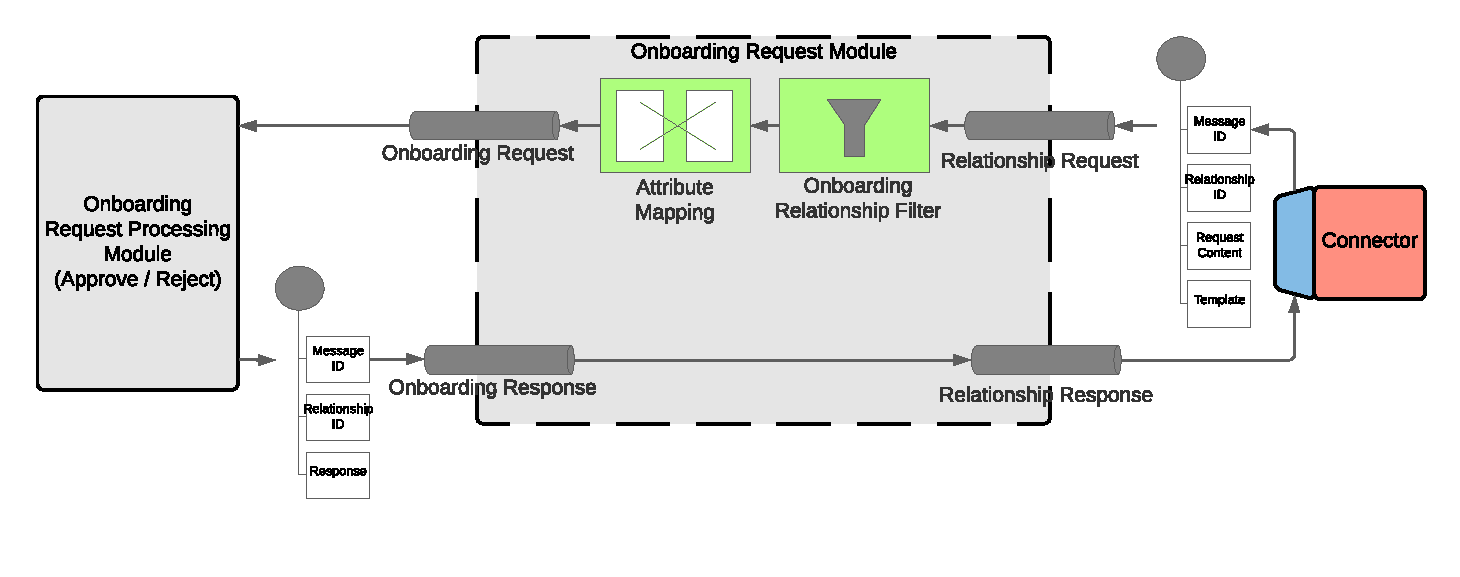
\includegraphics[scale=0.6]{Diagrams/Integration Architecture 1/Technological Integration/7. Onboarding Request Module.pdf}
\end{center}

Eventually, the user scans the QR code, fills in the attributes and submits a relationship request. The request is received by the connector, forwarded to the messaging adapter and published on the "Relationship Request" channel. The message contains a relationship ID created by the IMP server to uniquely identify the request and the resulting relationship. It also contains the request content with attributes shared by the user and the template the request originated from. Messages on the "Relationship Request" channel are consumed by the "Onboarding Request Module". As in the previous example, message translators are included to construct a canonical data model for the module. A message filter only lets messages trough which contain templates of type onboarding. The message translator connected to the "Onboarding Request" channel translates attributes shared by the user from the IMP data model to the OZG data model.

Based on the attributes the user shares, the OZG system has to decide if the relationship should be established or not. As this process heavily depends on the use case of the relationship and on the service provider, the messaging system expects the SP to add a module called "Onboarding Request Processing Module" which consumes the request and responds with either approve or reject on the "Onboarding Response" channel. To correlate the response to the request, the message also has to contain the relationship ID. The "Onboarding Request Module" forwards the response to the "Relationship Response" channel, where the connector will further interact with the IMP system to either establish or cancel the relationship.

\subsection{Onboarding Relationship Module}

\begin{center}
    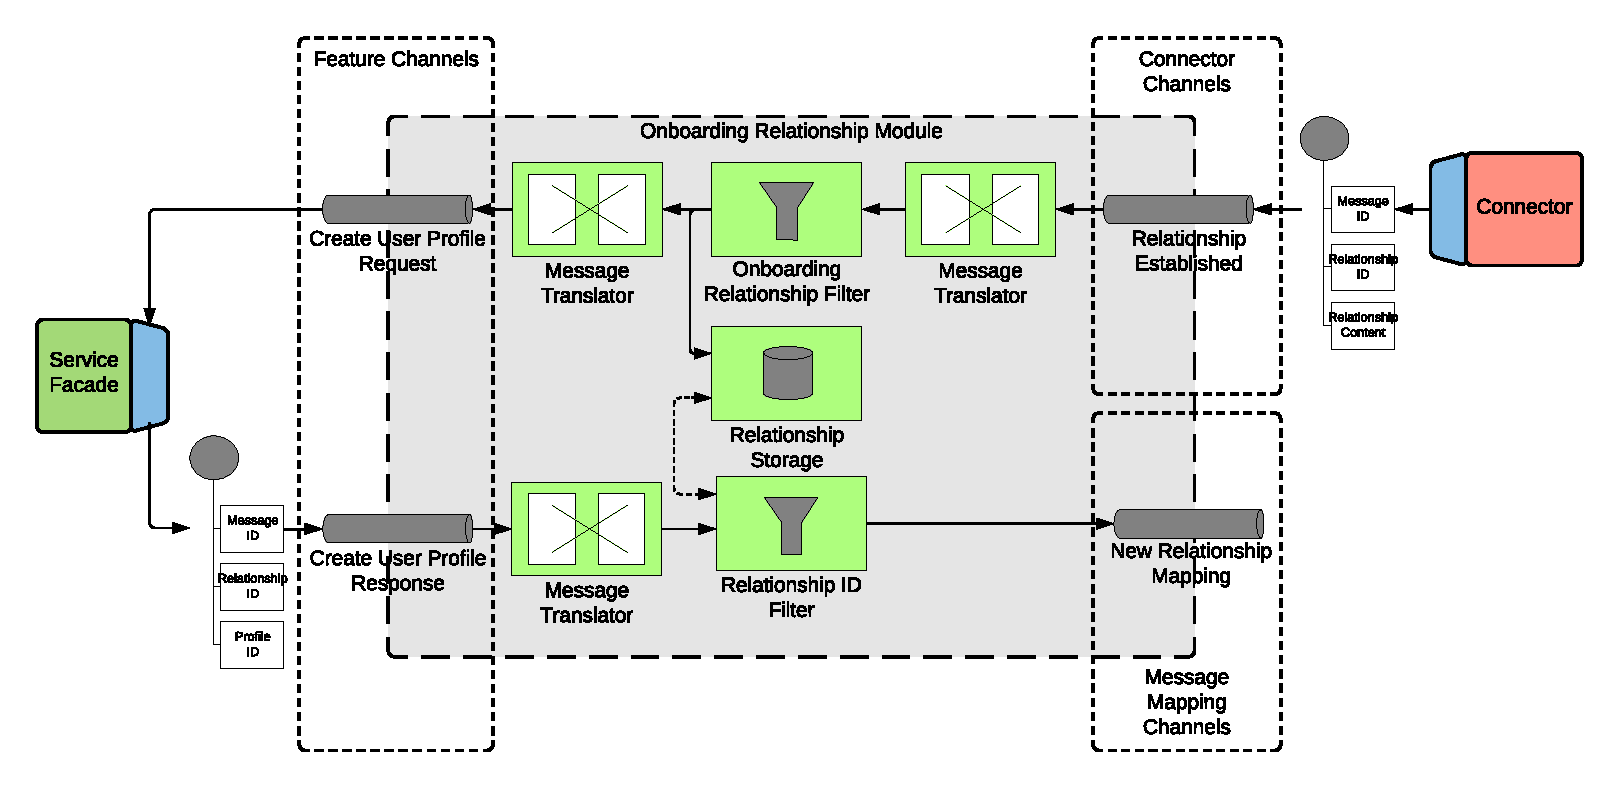
\includegraphics[scale=0.6]{Diagrams/Integration Architecture 1/Technological Integration/8. Onboarding Relationship Module.pdf}
\end{center}

If the user did not retract his relationship request before the OZG system accepted it, the relationship is established and the connector receives a corresponding notification which the messaging adapter publishes on the "Relationship Established" channel. The message contains the ID of the established relationship along with all attributes shared by the user. The "Onboarding Relationship" module consumes messages from the channel and is responsible for maintaining the state of onboarding relationships. In this case, the module only processes the establishing of relationships, it could however be expanded to also process terminations of relationships.

Message translators are inserted again for creating a canonical data model.

The module processes an established relationship by initiating the creation of a new user profile. First, a message filter lets trough only messages of the onboarding type. Afterwards, each message is stored in a "Relationship Storage" database and published on the "Create User Profile Request" channel. However, before publishing the message, a message translator maps attributes form the IMP data model to the OZG data model.

To create a user profile, a messaging adapter attached to the service facade of the administration portal consumes messages from the "Create User Profile Request" channel and issues the corresponding requests to the service facade for creating a new user profile based on the attributes stored in the relationship content. After successful creation of the user profile, the messaging adapter publishes a response message on the "Create User Profile Response" channel which contains the relationship ID and the newly created user profile ID.

As responses to requests from other modules might be published on this channel, the "Onboarding Relationship" module filters all messages which do not contain a relationship ID stored in the "Relationship Storage". The module then publishes the response on the "New Relationship Mapping" channel.

\subsection{Relationship Mapping Module}

\begin{center}
    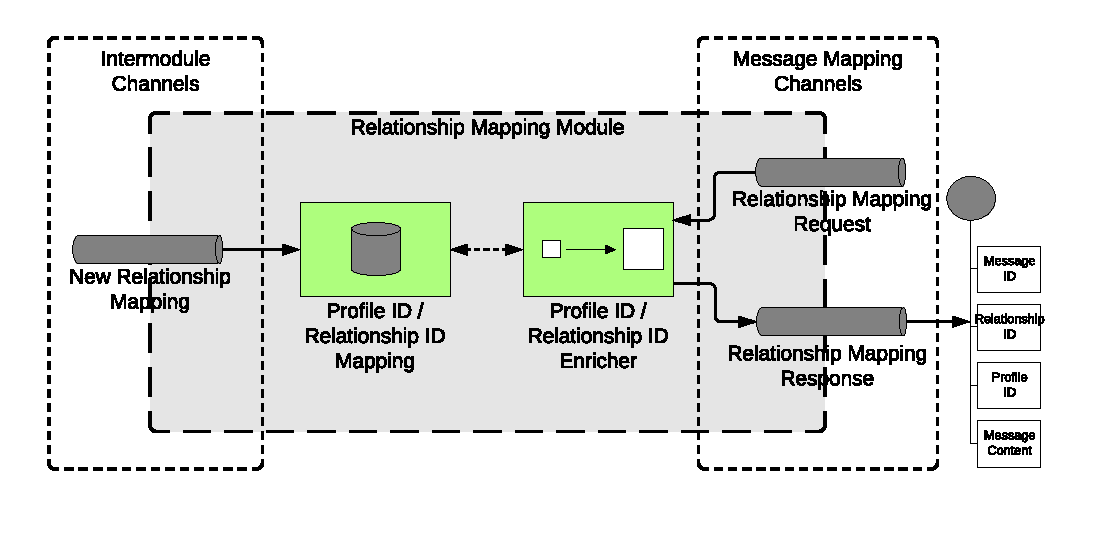
\includegraphics[scale=0.6]{Diagrams/Integration Architecture 1/Technological Integration/9. Relationship Mapping.pdf}
\end{center}

Trough the "New Relationship Mapping" channel, the "Relationship Mapping" module receives the message sent by the previously described module. Purpose of the "Relationship Mapping" module is to map relationships to corresponding entities in the existing system architecture. In this case, relationships are mapped to user profiles and vice versa using relationship IDs and user profile IDs. The message consumed trough the "New Relationship Mapping" channel is stored in a database for enabling future translation between the contained relationship ID and user profile ID. Using the "Relationship Mapping Request" channel, modules can request the "Relationship Mapping" module to add a user profile ID for a given relationship ID and vice versa.

Using messaging for this form of database access enables modules to stay unaware of the complexities of the underlying data storage mechanisms. An alternative would be for modules to use the database as a shared database.

\subsection{Message Mapping Module}

\begin{center}
    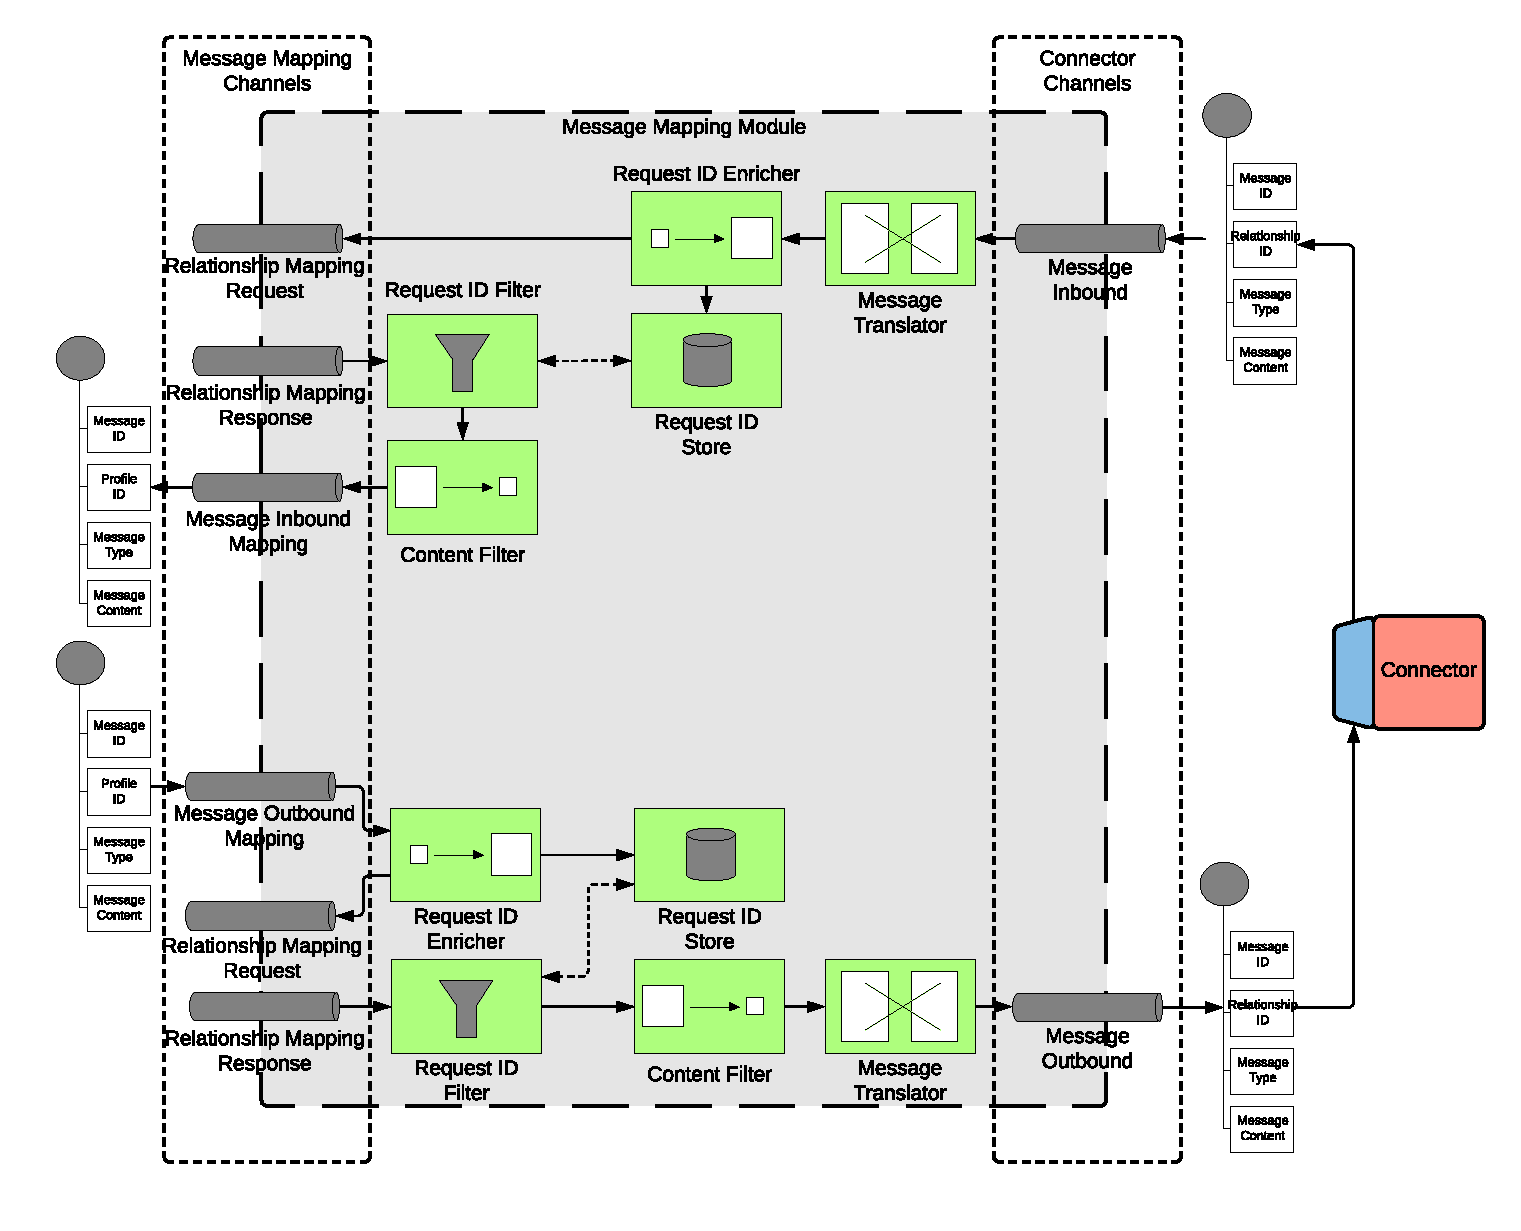
\includegraphics[scale=0.6]{Diagrams/Integration Architecture 1/Technological Integration/10. Message Mapping Module.pdf}
\end{center}

Using the previously defined "Relationship Mapping" module, the "Message Mapping" module has the purpose of translating the relationship ID of all inbound messages to the corresponding user profile ID and translating the user profile ID of all outbound messages to the corresponding relationship ID. As a result of that, on the left side, messages coming from or going to the existing system architecture, messages contain identification of the known user profile entity instead of the unknown relationship entity. On the right side, messages coming from or going to the IMP system contain identification of the known relationship instead of the unknown user profile.

Incoming messages on the "Message Inbound" channel are consumed by the module and translated by a message translator to a canonical data model. In order for the module to identify a response after publishing the message on the "Relationship Mapping Request" channel, a content enricher adds a unique request ID to the message and stores the ID in a database. Only messages on the "Relationship Mapping Response" channel containing a request ID stored in the database are let trough by the request ID message filter. As the following systems will process the inserted user profile ID instead of the relationship ID, a content filter removes relationship IDs from the message before publishing it on the "Message Inbound Mapping" channel.

Outbound messages on the "Message Outbound Mapping" channel are processed similar to inbound messages. The difference being, that the user profile ID contained in the message is replaced by the corresponding relationship ID.

\subsection{Attribute Change Message Module}

\begin{center}
    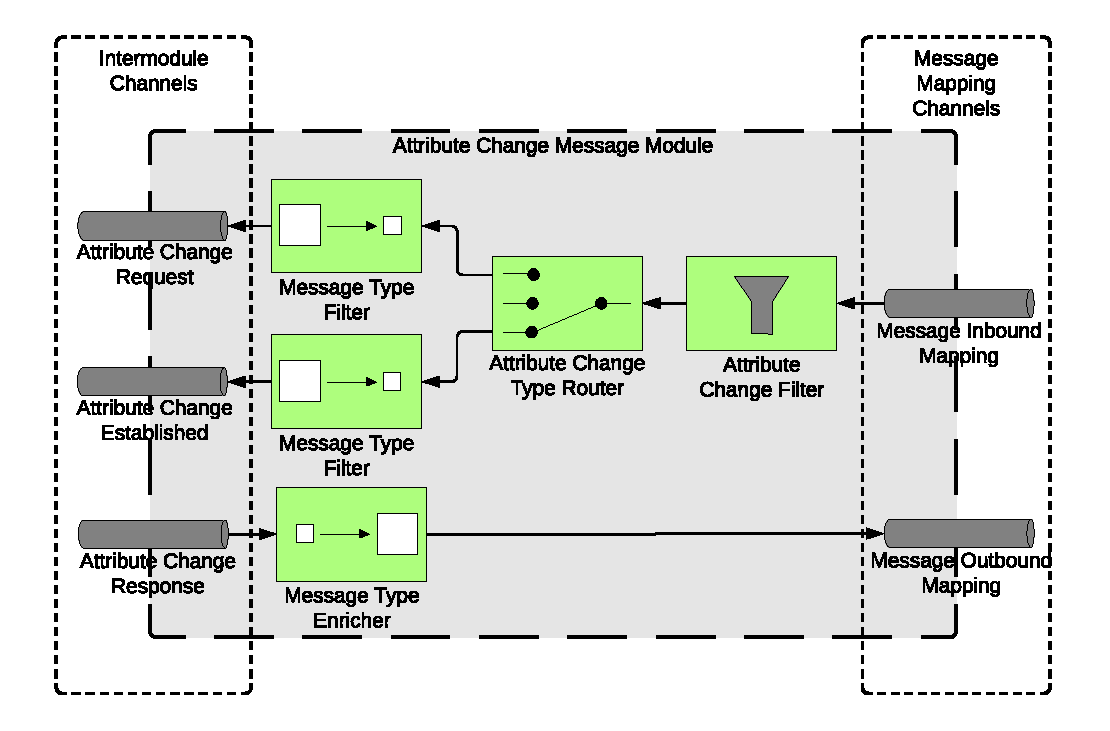
\includegraphics[scale=0.6]{Diagrams/Integration Architecture 1/Technological Integration/11. Attribute Change Message Module.pdf}
\end{center}

For the messaging system to process messages being exchanged as part of relationships, message modules can be added. Their purpose is to map messages of certain types on the "Message Inbound Mapping" channel to individual message type channels so that modules can process them. They also map messages of the individual message type channels to the "Message Outbound Mapping" channel to so that the connector can submit them.

In this case, an "Attribute Change Message Module" is included, which processes messages related to the attribute change process. Messages exchanged trough IMP relationships can have arbitrary content, however, the messages are assumed to contain a message type attribute and a message content attribute. Based on the message type attribute, a message filter can let messages trough which contain a message type attribute correlating to an attribute change process. Based on the type of a message, a content based message router then copies each message to a datatype channel. In this case, messages of type attribute change request and attribute change established are distinguished. Corresponding to that, two data type channels exist. As based on the channel, a message is placed, its message type can be inferred, content filters remove the message type attributes.

Outbound messages related to the attribute change process are consumed on data type channels. In this case, it is only one "Attribute Change Response" channel. A content enricher adds a message type attribute correlating to the channel the message was placed on. This is required in order for the IMP client to properly interpret the message. After that, the message is published on the "Message Outbound Mapping" channel.

\subsection{User Profile Attribute Change Request Module}

\begin{center}
    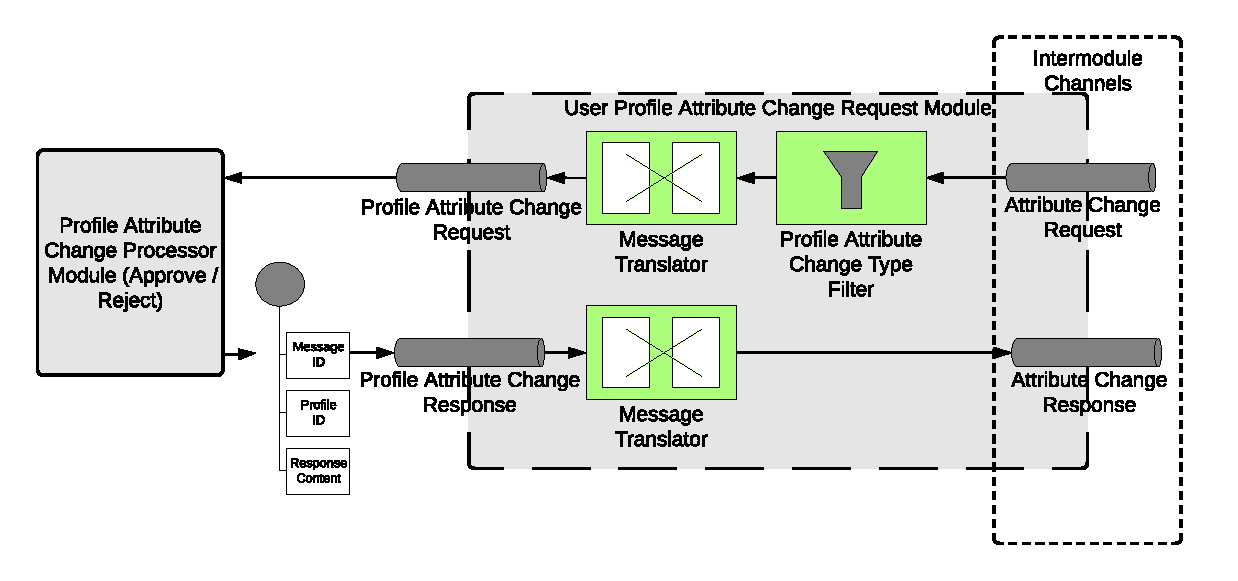
\includegraphics[scale=0.6]{Diagrams/Integration Architecture 1/Technological Integration/12. Attribute Change Request Module.pdf}
\end{center}

To process incoming attribute change requests for profiles, a "User Profile Attribute Change Request" module is included which consumes messages from the "Attribute Change Request" channel. Messages arriving on the "Attribute Change Request" channel were mapped form a relationship ID to a user profile ID in an earlier integration step. Depending on the use case of the service provider, not all user profiles should be processed in the same way. Therefore, message filters are inserted, which are able to distinguish possible "types" of user profiles based on the user profile ID. It would also be possible to include an additional module, which is able to request user profile type information from the existing systems, separating messages on the "Attribute Change Request" channel appropriately. For example, user profiles for businesses could exist, where processing of attribute change requests requires a more through and manual verification by employees. 

In the example at hand, however, only one module processes attribute change requests. To translate the canonical data model into the data model of the OZG, a message translator is included. This concerns especially the attributes shared as part of the attribute change request.

Similar to the "Onboarding Request Module", the decision whether to approve or reject an attribute change is specific to the service provider. Therefore, the SP is expected to include a "Profile Attribute Change Processor" module, which based on the user profile ID and the shared attributes decides to approve or reject the request. The response is published to the "Attribute Change Response" channel and besides the response, contains the user profile ID.

\subsection{User Profile Attribute Sync Module}

\begin{center}
    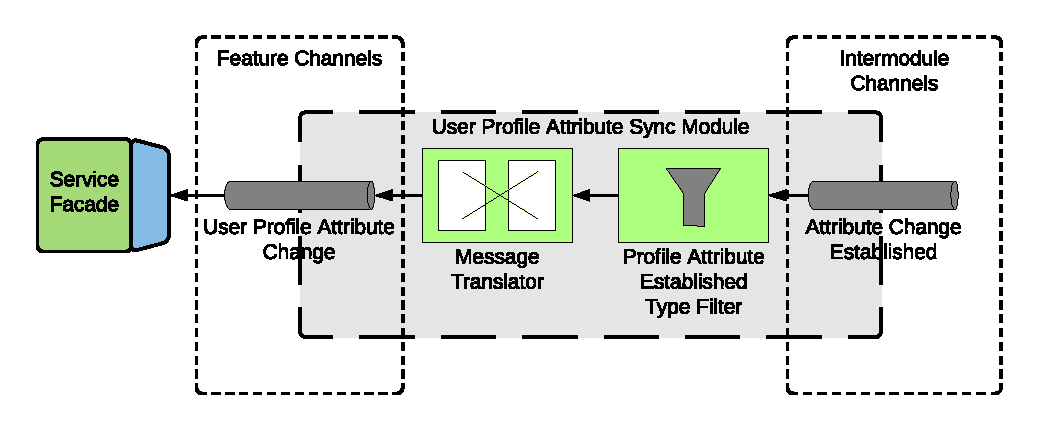
\includegraphics[scale=0.6]{Diagrams/Integration Architecture 1/Technological Integration/13. User Profile Attribute Sync Module.pdf}
\end{center}

If the user did not cancel the attribute change request before the OZG system accepted, the attribute change is established. The connector is notified trough a message, which eventually by processed by the "User Profile Attribute Change Message" module described earlier and published on the "Attribute Change Established" channel.

The "User Profile Attribute Sync" module consumes messages from the "Attribute Change Established" channel. Similar to the "User Profile Attribute Change Request" module, a message filter is inserted for distinguishing possible user profile types based on the user profile ID. A message translator is inserted to translate the message content to the OZG data model. This concerns especially the attributes shared as part of the attribute change established message.

\subsection{Mail Message module}

\begin{center}
    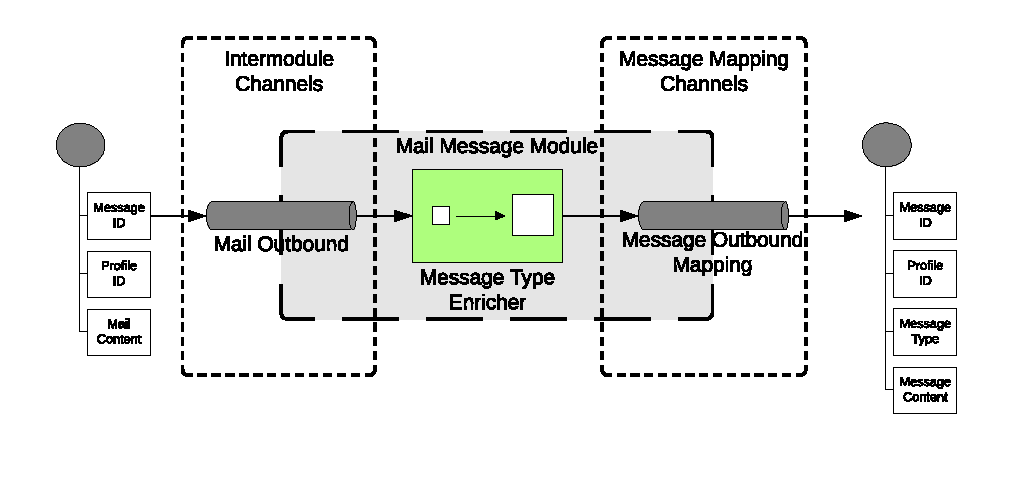
\includegraphics[scale=0.6]{Diagrams/Integration Architecture 1/Technological Integration/14. Mail Message Module.pdf}
\end{center}

In order for the user to receive messages sent to his user profile trough the IMP client, mail messages are processed by the integration architecture. Similar to the "Profile Attribute Change Message" module, a "Mail Message" module is included, which maps messages on the "Mail Outbound" channel to the "Message Outbound Mapping" channel.

In this module, incoming mails from the IMP client could also be processed.

Before publishing messages on the "Message Outbound Mapping" channel, a content enricher adds the implicit message type of the channel as attribute in order for the IMP client to understand it. 

\subsection{Mail Module}

\begin{center}
    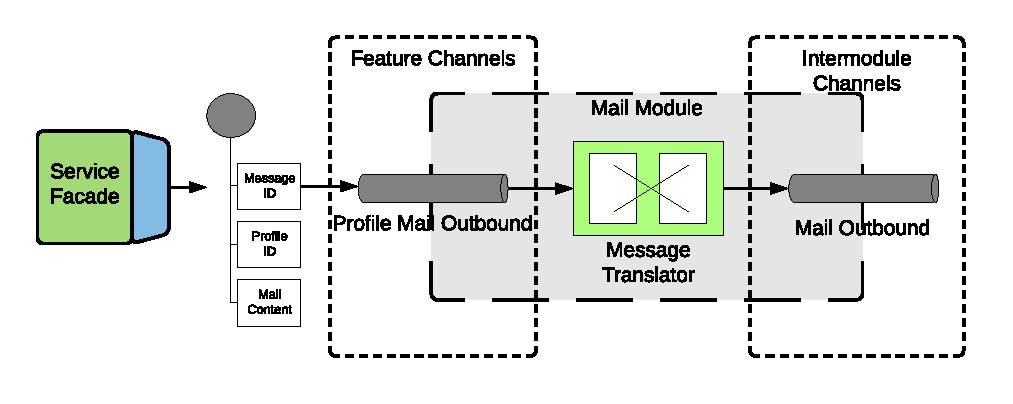
\includegraphics[scale=0.6]{Diagrams/Integration Architecture 1/Technological Integration/15. Mail Module.pdf}
\end{center}

A messaging adapter attached to the service facade is notified each time, a user profile connected to an IMP identity receives a mail and publishes a message on the "Profile Mail Outbound" channel. The message contains the ID of the profile which received the message and the content of the mail.

A "Mail" module is included which consumes the messages from the "Profile Mail Outbound" channel. A message translator is inserted, which translates the mails from the OZG data model to the IMP data model and publishes them on the "Mail Outbound" channel.

\subsection{Authentication Message Module}

\begin{center}
    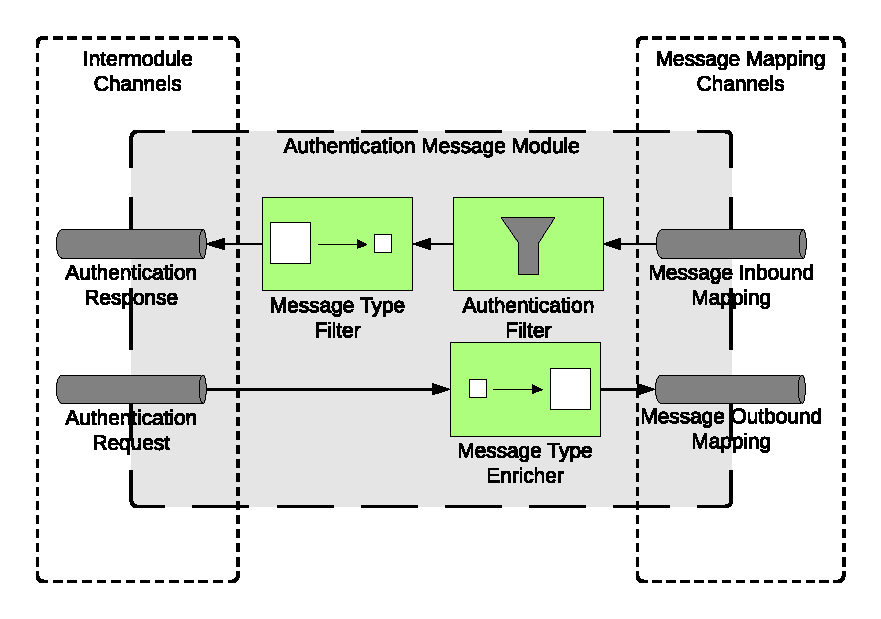
\includegraphics[scale=0.6]{Diagrams/Integration Architecture 1/Technological Integration/16. Authenticatin Message Module.pdf}
\end{center}

If the user creates a user profile using his IMP identity, it is possible to replace authentication using a password with authentication trough the IMP client. It is also possible to use the IMP client for two factor authentication.

In order to send and receive messages related to authentication, similar to previous message modules, an "Authentication Message" module is included which maps incoming messages on the "Message Inbound Mapping" channel to the "Authentication Response" channel and outgoing messages from the "Authentication Request" channel to the "Message Outbound" channel.

\subsection{Authentication Module}

\begin{center}
    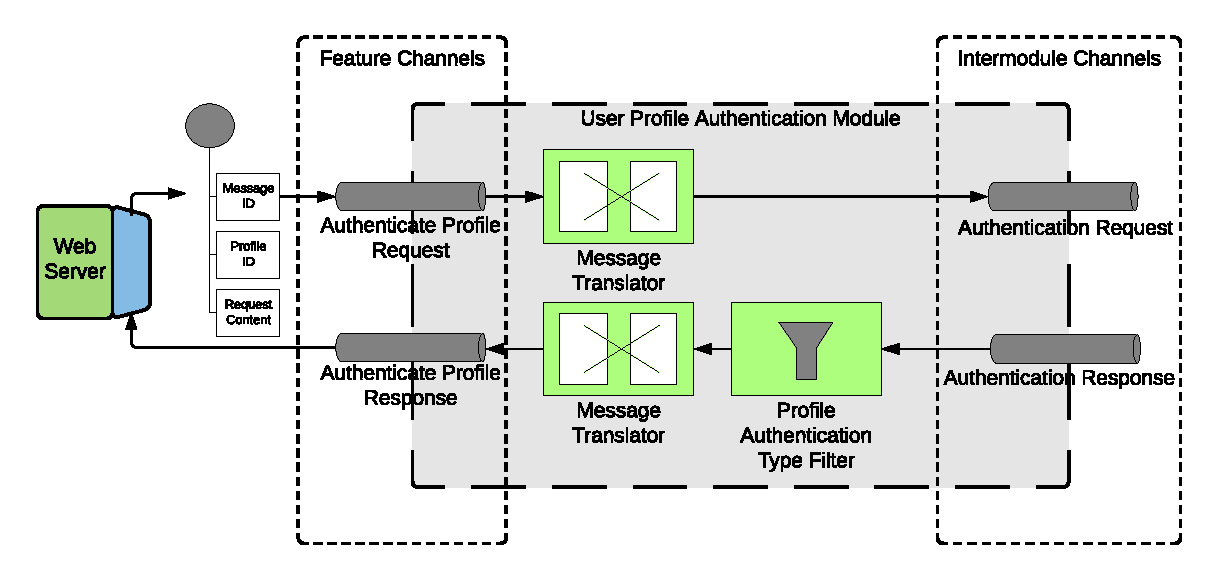
\includegraphics[scale=0.6]{Diagrams/Integration Architecture 1/Technological Integration/17. Authentication.pdf}
\end{center}

When the user visits the web page of the administration portal to apply for an administrative service, he will have to login. To utilize the IMP client for authentication, the web server can use a channel adapter to publish a authentication request concerning a user profile ID and a certain session ID. The adapter publishes a message on the "Authenticate" channel which contains the profile ID and a request content. Next to the session ID, the request content may also include information for presentation to the user like the current time or the IP address of the browser. Similar to previous modules, a message translator is inserted to translate the message to a canonical data model and publish it on the "Authentication Request Message".

Eventually, the IMP client sends a response as message, which the "Authentication Message" module publishes on the "Authentication Response" channel. Similar to previous modules, the service provider can use a message filter to process user profile types differently. After translating the message to the OZG data model, it is published on the "Authenticate Profile Response" channel. The channel adapter of the web server receives the message and based on the session ID contained in the response content can authenticate the browser session.